\section{Timing and Control Logic}
\label{timing}

This section outlines the necessary signals, timing considerations, and control circuitry for a synchronous SRAM.

\subsection{Signals}
\label{signals}
Top-Level Signals:
\begin{itemize}
\setlength{\itemsep}{0pt}
\item ADDR - address bus.
\item DATA - bi-directional data bus.
\item clk - the global clock.
\item OEb - active low output enable.
\item CSb - active low chip select.
\item WEb - active low write enable.
\end{itemize}

Internal Signals:
\begin{itemize}
\setlength{\itemsep}{0pt}
\item clk\_bar - enables the precharge unit.
\item s\_en - enables the sense amp during a read operation.
\item w\_en - enable the write driver during a write operation.
\item tri\_en and tri\_en\_bar - enable the data input tri-gate during a read operation.
\end{itemize}

\subsection{Timing Considerations}
\label{timing_params}

The main timing considerations for an SRAM are:
\begin{itemize}
\setlength{\itemsep}{0pt}
\item Setup Time - time an input needs to be stable before the positive/negative clock edge.
\item Hold Time - time an input needs to stay valid after the positive/negative clock edge.  
\item Minimun Cycle Time - time inbetween subsequent memory operations.
\item Memory Read Time - time from negative clock edge until valid data appears on the data bus.
\item Memory Write Time - time from negative clock edge until data has been driven into a memory cell.
\end{itemize}

\subsection{SRAM Operation}
\label{operation}

\begin{figure}[tb]
\centering
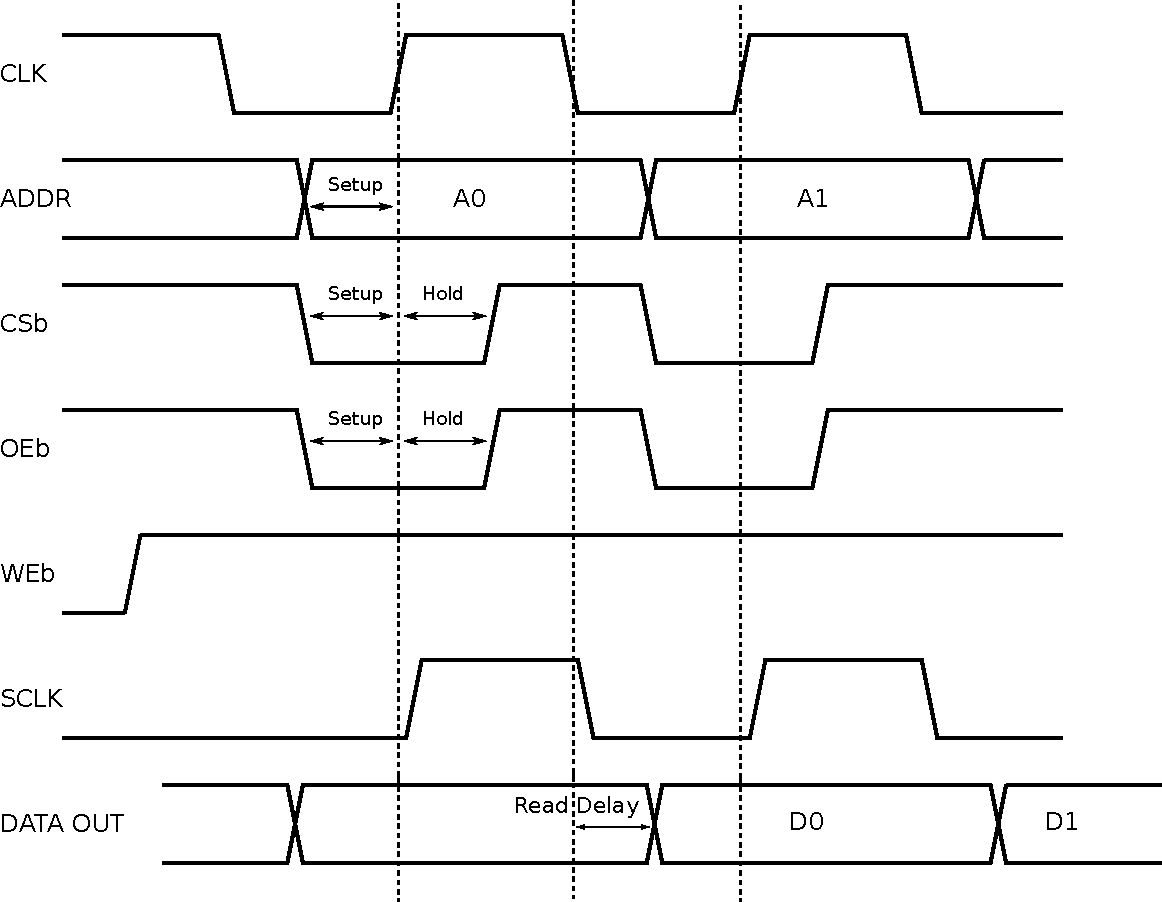
\includegraphics[scale=.85]{./figs/timing_read.pdf}
\caption{Timing diagram for read operation showing the setup, hold, and read times.}
\label{fig:read}
\end{figure}

Read Operation:
\begin{enumerate}
\setlength{\itemsep}{0pt}
 \item Before the clock transition (low to high) that initiates the read operation:
  \begin{enumerate}
	\item The chip must be selected (CSb low).
	\item The WEb must be high (read). 
	\item The row and column addresses must be applied to the address input pins (ADDR).
	\item OEb should be selected (OEb low).
   \end{enumerate}
 \item On the rising edge of the clock (CLK):
   \begin{enumerate}
	\item The control signals and address are latched into flip-flops and the read cycle begins. 
	\item The precharging of the bit lines starts.  
	\item The address bits become available for the decoder and column mux, which select the row and columns that we want to read from.
   \end{enumerate}
 \item On the falling edge of the clock (CLK):
   \begin{enumerate}
        \item Word line is driven onto the bitlines, the value stored in the memory cells pulls down one of the bitlines (bl if a 0 is stored, br if a 1 is stored).
	\item s\_en enables the sense amplifier which senses the voltage difference of the bit lines, produces the output and keeps the value in its latch circuitry.
	\item Tri-gate drives (tri\_en and tri\_en\_bar) the output data on data bus. Data remains valid on the data bus for a complete clock cycle.
   \end{enumerate}
\end{enumerate}


\begin{figure}[tb]
\centering
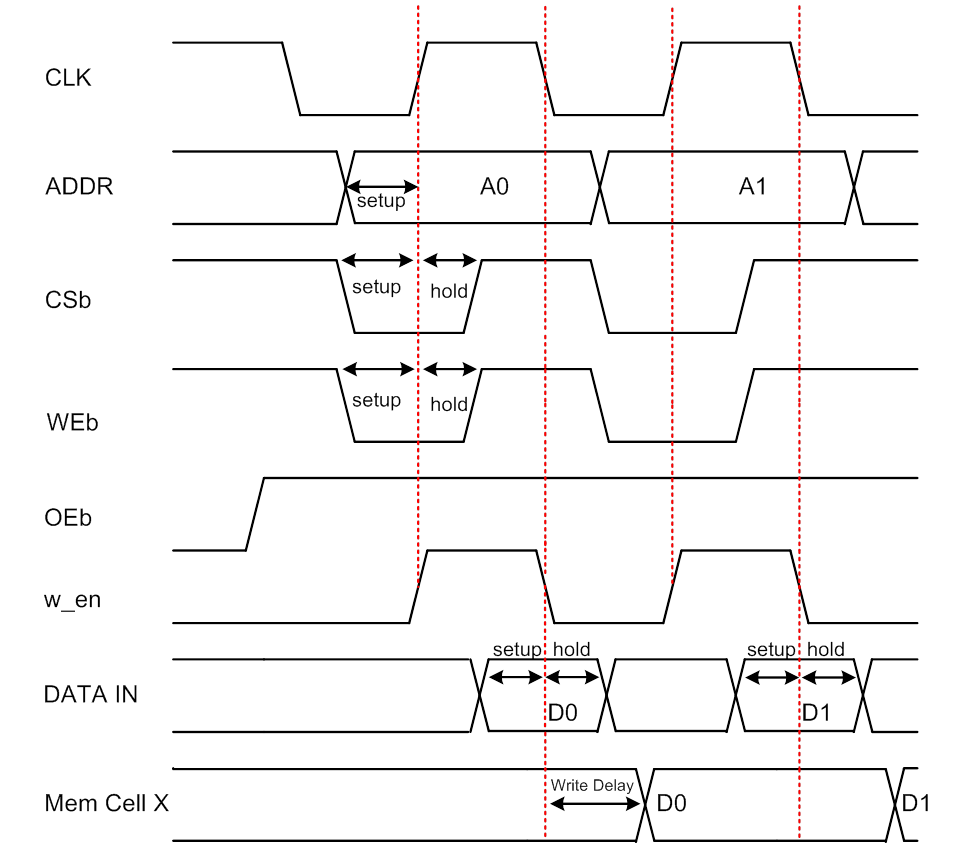
\includegraphics[scale=.9]{./figs/timing_write.pdf}
\caption{Timing diagram for write operation showing the setup, hold, and write times.}
\label{fig:write}
\end{figure}



Write Operation:
\begin{enumerate}
\setlength{\itemsep}{0pt}
 \item Before the clock transition (low to high) that initiates the write operation:
  \begin{enumerate}
	\item The chip must be selected (CSb low).
	\item The WEb must be low to enable the data input tristates.
	\item The row and column addresses must be applied to the address input pins (ADDR).
	\item OEb must be high (no output is available and sense amp disabled)
  \end{enumerate}
 \item On the rising edge of the clock (CLK):
   \begin{enumerate}
	\item OEb stays high (no output is available and sense amp disabled)
	\item The inputs addresses are latched into flip-flops, precharging starts, and the write operation begins.
	\item The address bits become available for the decoder and column mux, which select the row and columns that we want to write to.
  \end{enumerate}	         
 \item On the falling edge of the clock (CLK):
   \begin{enumerate}
	\item The data to be written must be applied to DATA and latched into flip-flops.
	\item w\_en enables the write driver, which drives the data input through the column mux and into the selected memory cells.  The write delay is the time from the negative clock edge until the data value is stored in the memory cell on node X.
   \end{enumerate}
\end{enumerate}


\subsection{Zero Bus Turnaround (ZBT)}
\label{sec:ZBT}

In timing of SRAM, during a read operation, data should be available after the clock edge while 
during a write, data should be set up before the clock edge. Due to this issue a wait state (dead cycle) is neccessary when SRAM switches 
from read mode to write mode. 
To avoide dead cycles in SRAM timing which slow down the operation and degrade the performance of SRAM, Zero Bus turnaround (ZBT) technique is used.
Using ZBT, during a write, data is set up after positive clock edge and before negative clock edge and input data is latched in negative edge flip-flops. 
Using ZBT, we will get a higher memory throughput and there is no waite states.
Figure~\ref{fig:write} shows the correct timing for input signals during the write opertion to avoide the wait states. 
Figure~\ref{fig:ZBT} shows how a write cycle is followed by a read cycle with no wait state through using ZBT.
Input address bits should be ready before positive edge to be loaded to positive edge flip-flops. Output data is ready to be loaded to data-bus during seconde half of cycle (after negative edge of clock) and 
input data should be ready before negative edge of clock to be loaded in negative edge  flip-flops.

\begin{figure}[h!]
\centering
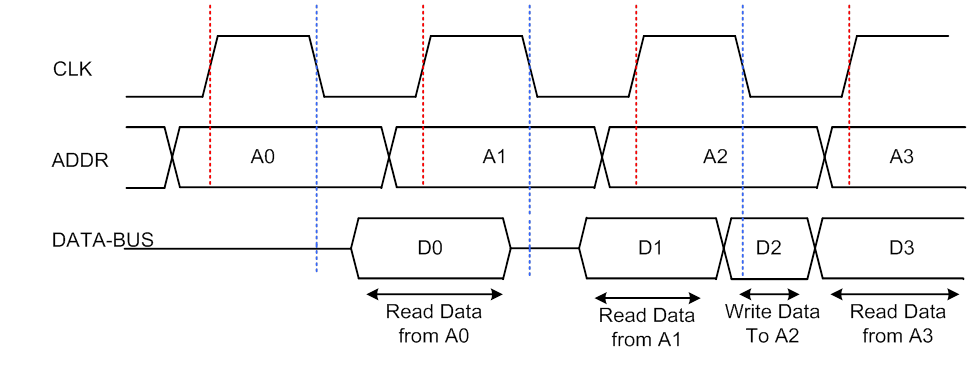
\includegraphics[scale=0.9]{./figs/ZBT.pdf}
\caption{(a) Zero Bus Turnaround timing.}
\label{fig:ZBT}
\end{figure}


\subsection{Control Logic}
\label{sec:control}



The control circuitry ensures that the SRAM operates as intended during a read or write cycle by enabling the necessary structures in the SRAM. 
As shown in Figure~\ref{fig:control}, the control logic takes three active low signals as inputs: chip select bar ($CSb$), 
output enable bar ($OEb$), and write enable bar ($WEb$). $CSb$ enables the entire SRAM chip. 
When $CSb$ is low, the appropriate control signals are generated and sent to the architecture blocks.  
Conversely, if $CSb$ is high then no control signals are generated and SRAM is turned off or disabled. 
The $OEb$ signal signifies a read operation; while it is low the value seen on the data bus will be an output from the memory. 
Similarly, the $WEb$ signal signifies a write operation. All of the input control signals are latched with master-slave flip-flops, 
ensuring that the control signal stays valid for the entire operation cycle. The control signal flip-flops use the normal clock to generate 
local signals used to enable or disable structures based on the operation. Address flip-flops are combined with global clock as well. 
In a standard write SRAM, switching from a read to a write operation results in a dead cycle. To avoid this dead cycle, Data flip-flops are 
latched with $clk\_bar$ in order to have a Zero Bus Turnaround (ZBT) memory. More details on ZBT timing are outlined in Section~\ref{sec:ZBT}. 
After all control signals are latched, they are ANDED with the $clk\_bar$ because the read/write circuitries should only be enabled after the precharging of 
the bitlines had ended on the negative edge of the clock. The $w\_en$ signal enables the write driver during a write to the memory .The $s\_en$ signal 
is generated using a Replica Bitline ($RBL$) to enable the sense amplifier during a read operation. Details on $RBL$ architecture are outlined in section~\ref{sec:RBL}. 
$tri\_en$ and $tri\_en\_bar$ enable the tristates during read in order to drive the outputs onto the data bus. 
Table~\ref{table:control} shows the truth table for the control logic. The $s\_en$ signal to enable the sense amplifier is 
true when $(CS  .  OE  .  Clk\_bar)$ is true. Similarly, write driver enable signal, $w\_en$, is true when $(CS  .  WE .  clk\_bar)$ is true.  
$tri\_en$ and $tri\_en\_bar$ are true when $\neg(OEb\_bar  |  clk)$ and $\neg(OEb  .  clk\_bar)$ are true, respectively.
\begin{figure}[h!]
\centering
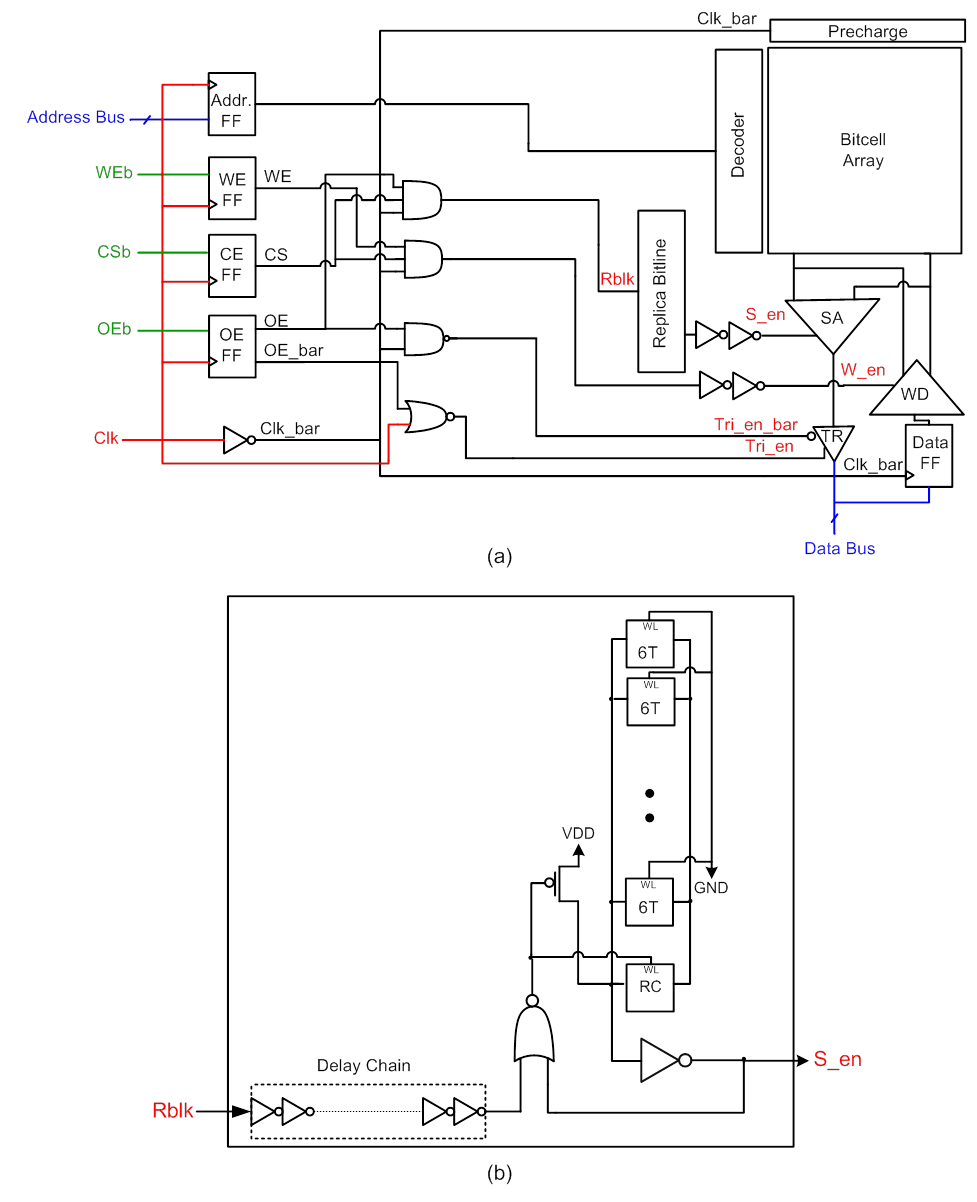
\includegraphics[scale=1]{./figs/control_logic.pdf}
\caption{(a) Control Logic diagram and (b) Replica Bitline Schematic.}
\label{fig:control}
\end{figure}



\begin{table}[h!] 
  \begin{center}
    \begin{tabular}{| c | c | c | c | c | c | c |}
    \hline
    Operation & \multicolumn{3}{|c|}{Inputs} & \multicolumn{3}{|c|}{Outputs}\\ \hline
     & CSb & OEb & WEb & s\_en & w\_en & tri\_en\\ \hline
    READ & 0 & 0 & 1 & 1 & 0 & 1\\ \hline
    WRITE & 0 & 1 & 0 & 0 & 1 & 0\\ \hline
    \end{tabular}
  \end{center}
  \caption{Generation of control signals.}
  \label{table:control}
\end{table}
	 
	 
\subsection{Replica Bitline Delay}
\label{sec:RBL}


	 
In SRAM read operation, discharging the bitline is the most time consuming procedure. 
Generally, sense amplifier amplifies the small voltage difference on the bitlines at the proper sense timing, 
to realize high-speed operation. Therefore, the timing for sense amplifier ($s\_en$) is extremely important for the high speed and low power SRAM. 
If the $s\_en$ arrives early before the bitline difference reaches the sense amplifier input transistors offset voltage, 
a read functional failure may occur. Contrarily, a late-arrived $s\_en$ would consume more unnecessary time, thereby wasting the power. 
The conventional way of generating $s\_en$ signal is to use a replica bitline ($RBL$). $RBL$ as shown in ~\ref{fig:RBL} consists of a column of SRAM cells (dummy cells), 
which track the random process variation in array. $RBL$ is presented for matching the delay of the activation of the 
sense amplifier with the delay of the propagation of the required voltage swing at the bitlines. 
In $RBL$ technique, delay driven memory cell in control path is same as read path. Therefore the 
delay shift of control path according to the Process, Voltage and Temperature (PVT) variation is same ratio as that of read path. 
The $RBL$ technique attains self-timed tracking with optimal $s\_en$ timing according to PVT variation. 
Using replica circuits, the variation on the delay of the sense amp activation and bitline swing is minimized.

\begin{figure}[h!]
\centering
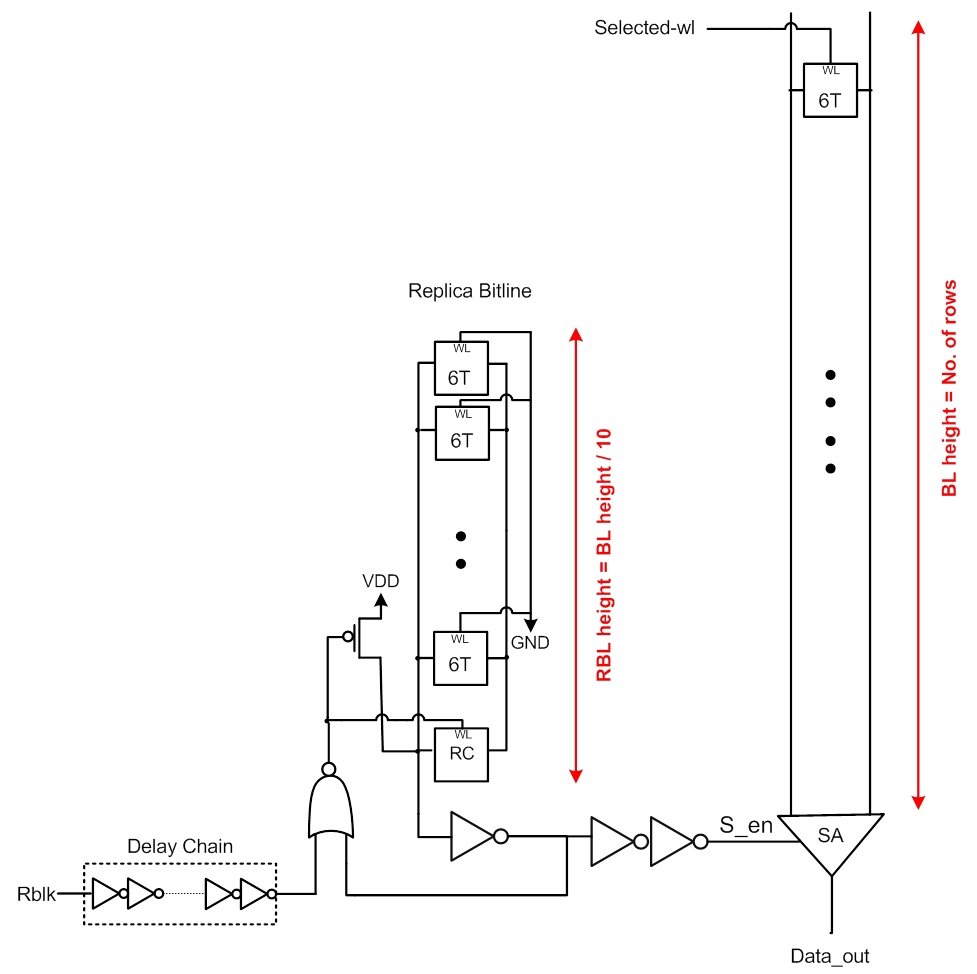
\includegraphics[scale=.9]{./figs/replica_bitline.pdf}
\caption{Replica Bitline Schematic}
\label{fig:RBL}
\end{figure}
 
$RBL$ technique uses a Replica Cell ($RC$) driving a short bitline signal. The short bitline\'s capacitance is set to be a 
fraction of the main bitline capacitance (e.g. one tenth). This fraction is determined by the required bitline swing 
(bitline voltages larger than offset voltage at input transistors of sense amplifier) for proper sensing. So in SRAM, an 
extra column block is converted into the replica column whose capacitance is the desired fraction of the main bitline. 
Therefore, its capacitance ratio to the main bitlines is set purely by the ratio of the geometric lengths (e.g. one tenth). 
The $RC$ is hard wired to store a zero such that it will discharge the $RBL$ once it is accessed. 
Because of its similarity with the actual memory cell (in terms of design and fabrication) the delay of $RBL$ tracks the delay of 
real bitlines very well and can be made roughly equal.  Figure ~\ref{fig:RC} shows the schematic of the 6T replica cell. 
The timing for $s\_en$ is generated as follows. At first, the $RBL$ and the normal bitlines are precharged to VDD. 
Next, selected memory cells and $RC$ are activated.  $RC$ draws the current from the $RBL$ and normal bitlines are 
also discharged through the accessed cell. Discharged swing on $RBL$ is inverted and then buffered to generate the signal to enable the sense amplifier.

	  
\begin{figure}[h!]
\centering
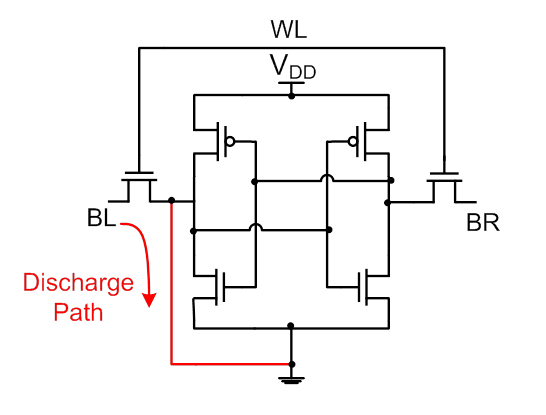
\includegraphics[scale=1]{./figs/replica_cell.pdf}
\caption{Replica Bitline Schematic}
\label{fig:RC}
\end{figure}




\subsection{Timing and Power Characterizer}
\label{characterizer}

The section will provide an explanantion of the characterizer that will generete spice stimuli for the top-level SRAM and perform spice timing simulations to determine the memory setup\&hold times, the write delay, and read delay.  It will also provide a spice power estimate.  

